% TODO chequear la forma de referirse a NUESTRO algoritmo sin decir la palabra NUESTRO :s
%% TODO: Ojo, a partir de acá hablamos en pasado. Deberíamos ser consistentes,
%% por como arrancamos en el resuemen, la intro y por lo que dice la mina
%% deberiamos usar el presente o eso de "se plantea, se define, etc..."

\section{Comparación con IFTrace}
\label{sec:iftrace}

El algoritmo de seguimiento IFTrace, propuesto por \citeauthor*{IFTrace}, es un
algoritmo robusto que soporta cambios de iluminación y forma, oclusiones y se
centra en hallar características representativas de la textura de los objetos a
seguir. Es capaz de recuperarse de errores menores y permite el seguimiento de
múltiples objetos a la vez.

Un algoritmo de este tipo podría proporcionar una solución al problema. Para
comprobarlo, se llevaron a cabo algunas pruebas utilizando un video sintético
creado para este fin, y un video real de un partido de fútbol. En las Figuras
\ref{fig:sample-happy-occluded} y \ref{fig:sample-boca} pueden observarse los
primeros cuadros de cada video. Pueden apreciarse a simple vista las marcadas
diferencias entre ambos videos, como por ejemplo la resolución de la imagen y
el tamaño y la complejidad de los objetos de inteŕes.

\begin{figure}[H]
    \centering
    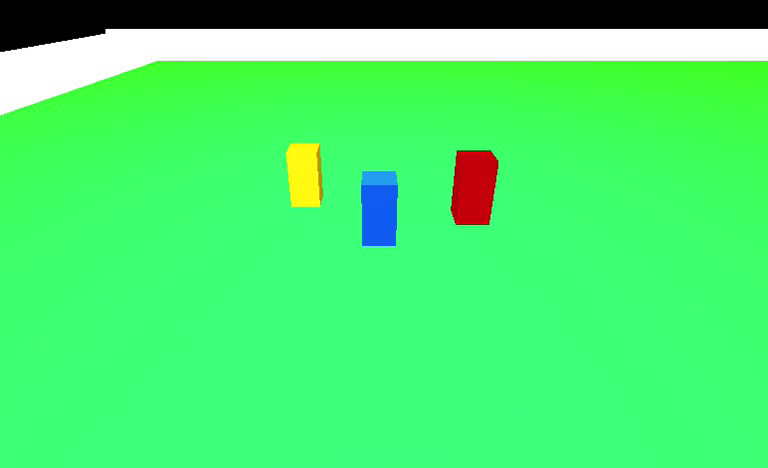
\includegraphics[width=\linewidth]{./images/sample_happy_occluded.png}
    \caption{Muestra de un cuadro del video sintético de prueba.}
    \label{fig:sample-happy-occluded}
\end{figure}

\begin{figure}[H]
    \centering
    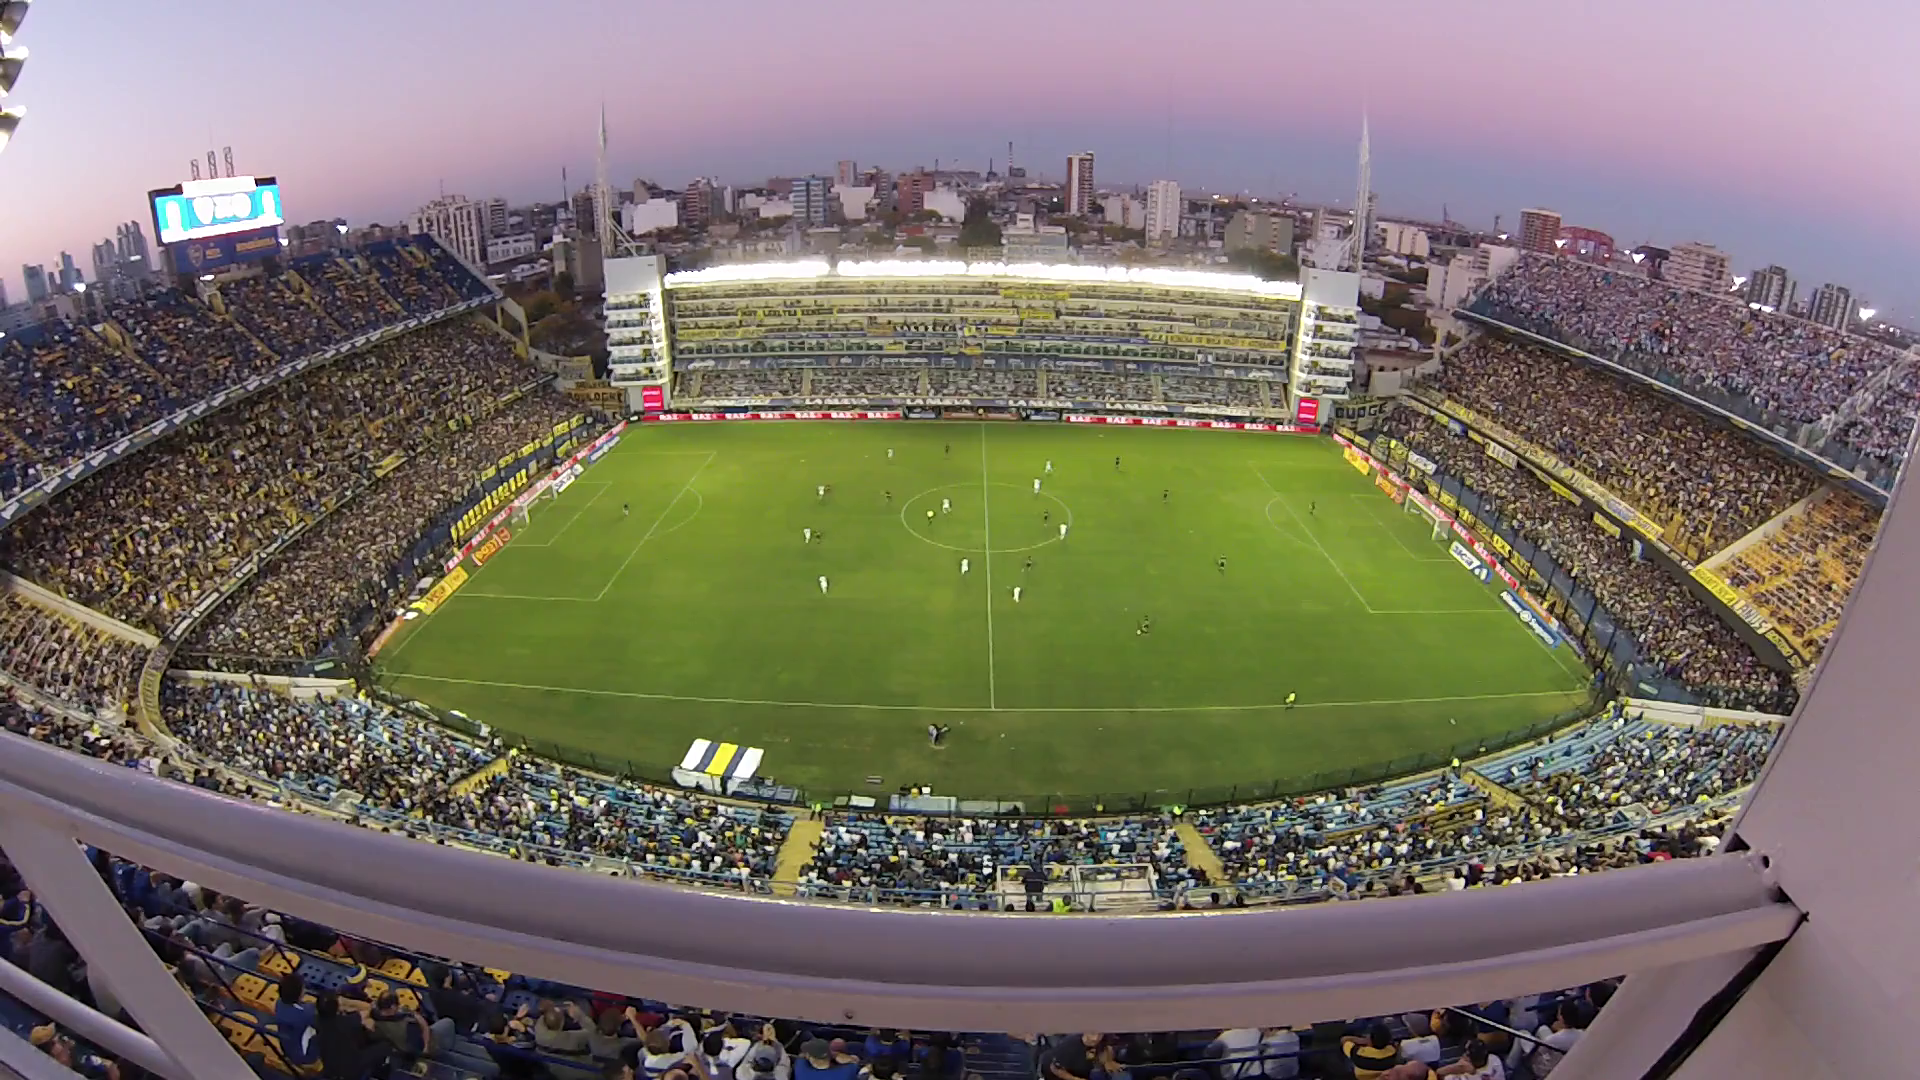
\includegraphics[width=\linewidth]{./images/sample_boca.png}
    \caption{Muestra de un cuadro del video real de un partido de fútbol.}
    \label{fig:sample-boca}
\end{figure}

Como se puede ver en la Figura \ref{fig:happy-occluded-iftrace}, IFTrace logra
un correcto seguimiento de múltiples objetos en el video sintético. También
puede observarse, en la Figura \ref{fig:boca-iftrace}, como sigue correctamente
a un jugador en el video real. Sin embargo, el seguimiento sólo es exitoso
durante unos pocos cuadros, ya que, en el cuadro 17, el algoritmo cae en un
error del cual sólo una corrección manual puede sacarlo. Este tipo de correción
semi-supervisada no está contemplada en el algoritmo de IFTrace.

\begin{figure}[H]
    \centering
    \begin{tabular}{cccc}
        \subfloat[Cuadro 1]{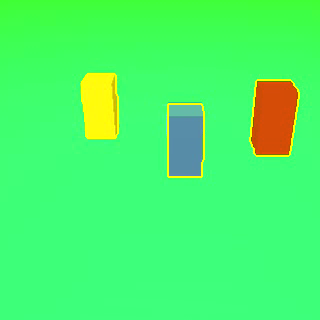
\includegraphics[width = 1.5in]{./images/cropped_happy_occluded_00001.png}} &
        \subfloat[Cuadro 5]{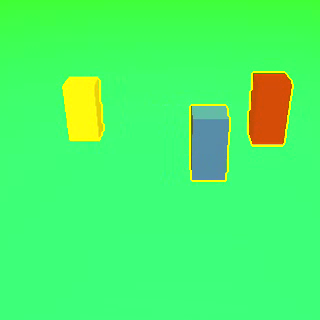
\includegraphics[width = 1.5in]{./images/cropped_happy_occluded_00005.png}} &
        \subfloat[Cuadro 8]{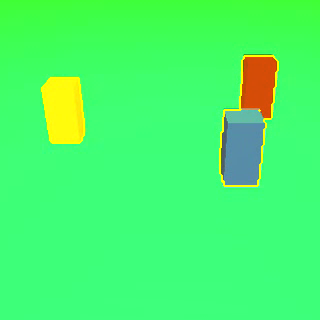
\includegraphics[width = 1.5in]{./images/cropped_happy_occluded_00008.png}} &
        \subfloat[Cuadro 12]{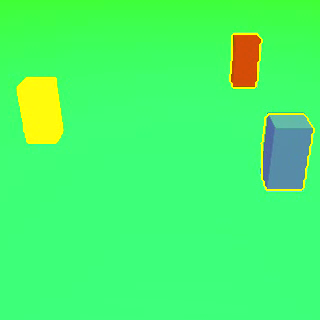
\includegraphics[width = 1.5in]{./images/cropped_happy_occluded_00012.png}}
    \end{tabular}
    %% NASTY hack to make refernce work with figures and subfigures, put \label inside \caption env, little bird told me
    \caption{IFTrace funcionando en una secuencia de cuadros de video sintético.
    \label{fig:happy-occluded-iftrace}
    }
\end{figure}

\begin{figure}[H]
    \centering
    \begin{tabular}{cccc}
        \subfloat[Cuadro 9]{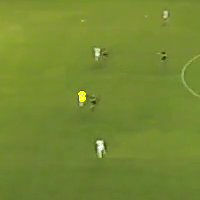
\includegraphics[width = 1.5in]{./images/cropped_boca_00009.png}} &
        \subfloat[Cuadro 12]{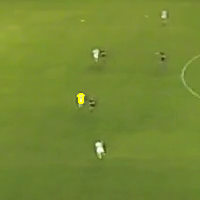
\includegraphics[width = 1.5in]{./images/cropped_boca_00012.png}} &
        \subfloat[Cuadro 14]{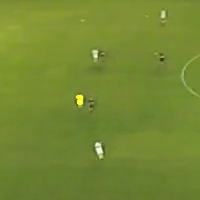
\includegraphics[width = 1.5in]{./images/cropped_boca_00014.png}} &
        \subfloat[Cuadro 17]{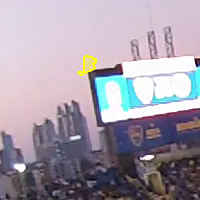
\includegraphics[width = 1.5in]{./images/cropped_boca_00017.png}}
    \end{tabular}
    %% NASTY hack to make refernce work with figures and subfigures, put \label inside \caption env, little bird told me
    \caption{Seguimiento de un jugador en un video real utilizando IFTrace.
    \label{fig:boca-iftrace}
    }
\end{figure}

\begin{figure}[H]
    \centering
    \begin{tabular}{cccc}
        \subfloat[Cuadro 1]{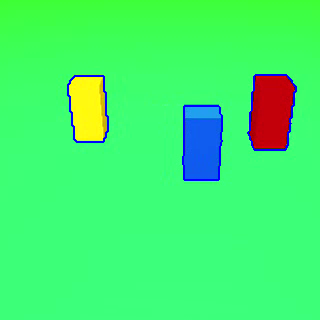
\includegraphics[width = 1.5in]{./images/cropped_processing2.png}} &
        \subfloat[Cuadro 5]{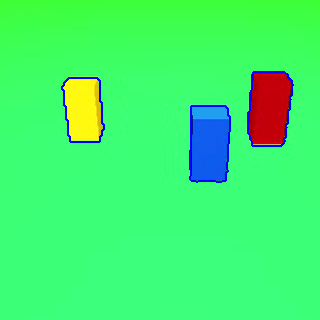
\includegraphics[width = 1.5in]{./images/cropped_processing5.png}} &
        \subfloat[Cuadro 8]{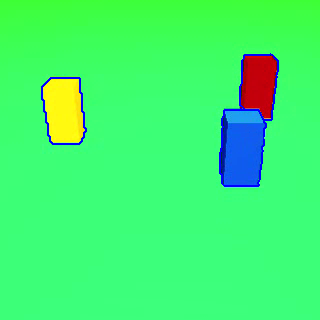
\includegraphics[width = 1.5in]{./images/cropped_processing14.png}} &
        \subfloat[Cuadro 12]{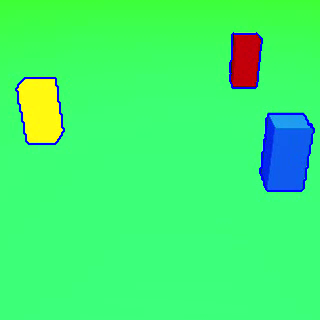
\includegraphics[width = 1.5in]{./images/cropped_processing25.png}}
    \end{tabular}
    %% NASTY hack to make refernce work with figures and subfigures, put \label inside \caption env, little bird told me
    \caption{El algoritmo de contornos activos modificado en funcionamiento en un video sintético.
    \label{fig:happy-occluded-activeContour}
    }
\end{figure}

\begin{figure}[H]
    \centering
    \begin{tabular}{cccc}
        \subfloat[Cuadro 2]{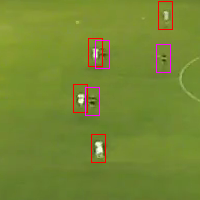
\includegraphics[width = 1.5in]{./images/cropped_rendered002.png}} &
        \subfloat[Cuadro 12]{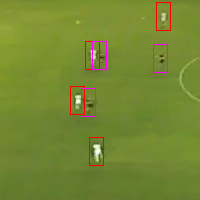
\includegraphics[width = 1.5in]{./images/cropped_rendered007.png}} &
        \subfloat[Cuadro 14]{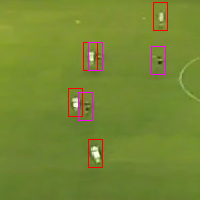
\includegraphics[width = 1.5in]{./images/cropped_rendered012.png}} &
        \subfloat[Cuadro 17]{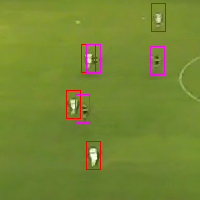
\includegraphics[width = 1.5in]{./images/cropped_rendered017.png}}
    \end{tabular}
    %% NASTY hack to make refernce work with figures and subfigures, put \label inside \caption env, little bird told me
    \caption{Seguimiento de los jugadores en un video real mediante el algoritmo de contornos activos modificado.
    \label{fig:boca-activeContour}
    }
\end{figure}

Como se puede observar en la Figura \ref{fig:happy-occluded-activeContour}, el
algoritmo propuesto en este trabajo logra seguir con éxito a los objetos de
interés en el video sintético. Además, también se obtiene un resultado positivo
en el video real en la situación en que IFTrace pierde al jugador, como puede
observarse en la Figura \ref{fig:boca-activeContour}.

\subsection{Evaluación de comportamiento}

Otro punto importante de comparación entre los dos algoritmos es su tiempo de
ejecución, es decir el tiempo que tarda en llevar a cabo su trabajo.  De
acuerdo a las mediciones realizadas con un video real de un partido de fútbol,
siguiendo a un solo jugador, el tiempo promedio que tarda IFTrace por cuadro es
6.962 segundos, mientras que el algoritmo implementado tiene un tiempo promedio
de 0.712 segundos. Se puede observar que se encuentra un orden magnitud por
debajo de IFTrace, incluso antes de realizar optimizaciones.
%% 6.9628571428571435 si quieren los decimales
%% TODO verificar nuestro numero!!!

Cabe destacar que ambos algoritmos podrían verse beneficiados de ciertas
optimizaciones, como ser por ejemplo la programación en GPU y la reducción de
operaciones de \textit{Input/Output} al almacenamiento secundario (disco duro).

% TODO Esto creo que probablemente terminemos sacandolo right? Que métrica podemos meter?!?!
% - Comparación de nuestros resultados vs los de ellos (Métrica: cantidad de jugadores perdidos por frame -- o si se nos ocurre una mejor ambas o esa)
